\section{Introduction}
\label{sec-introduction}

%Define the problem and the goal of the project
%Explain why the problem is important
%Summarize your approach and key results
%Outline the rest of the paper
Since the advent of the Internet, compute devices have become not only more
prolific but also varied - encompassing not only high performance compute
clusters but also general purpose computers and mobile systems.  Moreover, the
assumptions made about the security model of a system has changed drastically;
users can no longer be trusted, and devices have the potential to interact with
unknown and possibly untrustworthy hosts while communicating sensitive
information. For example, the boom in smartphones has caused a secondary
explosion in the mobile application industry, allowing users to log in to
various trusted systems (e.g. bank accounts, medical records and shopping
accounts) remotely.

However, the sudden increase in connectivity exposes users to adversaries that
may attempt to leverage these interactions in order to obtain confidential
information or disrupt the use of services or applications.

In response to these changes, there has been an increasing effort in developing
trusted computing platforms augmented with specialized hardware modules that
provide security features such as authentication and decryption/encryption. One
such security feature that remains a focus in trusted computing research is
protecting off-chip memory. Protecting off-chip memory includes maintaining
confidentiality of private data. Challenges in designing memory protection
mechanisms involves providing encryption primitives at a low cost (money, area,
power and design complexity), high throughput and low latency without
compromising security. Current work also focuses on memory protection schemes
for general purpose and high performance computing systems.  The domain of
memory protection in the mobile and embedded computing domains is relatively
less studied and poses interesting challenges.  Mobile and embedded devices
often operate under strict power and area constraints. Providing secure memory
protection while following the prescribed power and area constraints as well as
maintaining performance of the computing devices is an ongoing challenge.

\begin{enumerate}
  \item Characterizing the power overhead of the memory system is still an open
    problem - especially in the context of encryption.
  \item We use first order approximations to model the power overhead of
  \item On die termination - ODT
    encrypting data on the memory system.
  \item We verify that encrypted data has a significant power overhead \fixme{
    add numbers}
  \item Outline the paper's sections
\end{enumerate}

\begin{figure}[!htb]
  \centering
  \begin{subfigure}[b]{0.4\textwidth}
    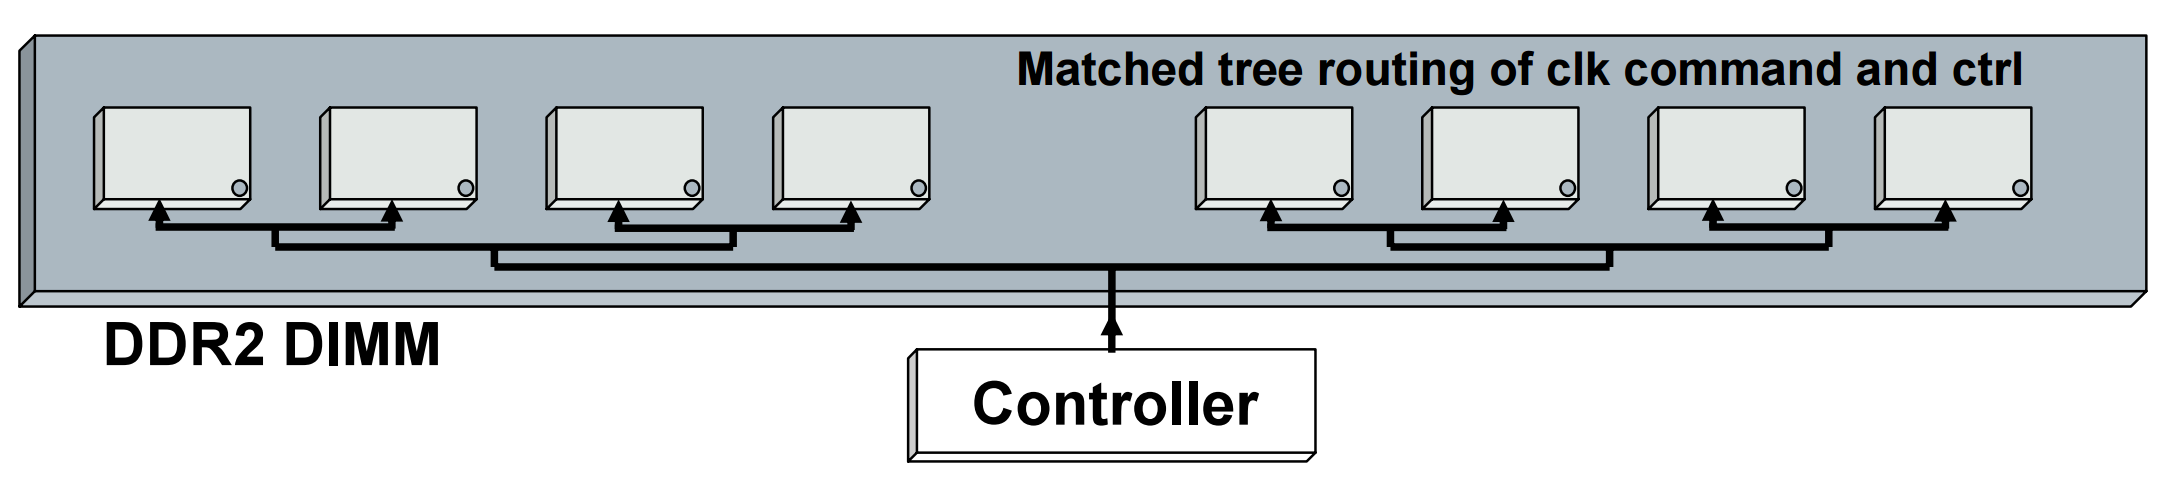
\includegraphics[width=\textwidth]{figs/ddr2-topology}
    \caption{ddr2}
    \label{fig:ddr2-chips}
  \end{subfigure}

  \begin{subfigure}[b]{0.4\textwidth}
    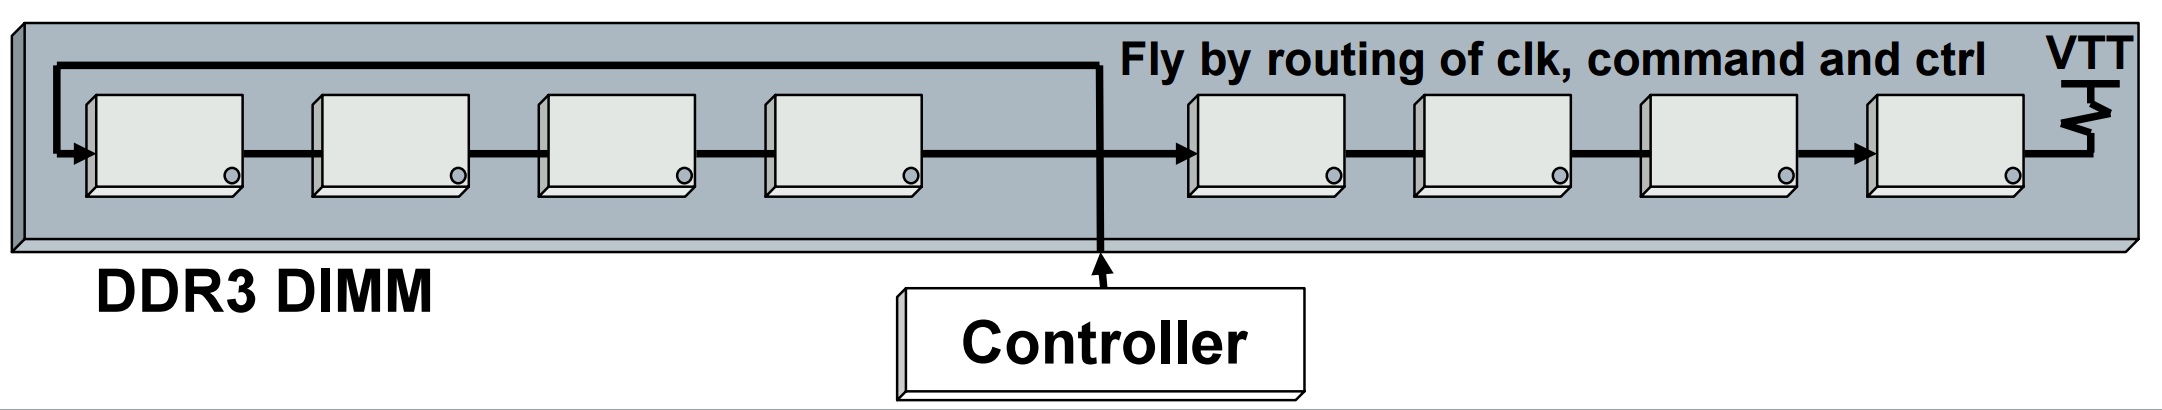
\includegraphics[width=\textwidth]{figs/ddr3-topology}
    \caption{ddr3}
    \label{fig:ddr3-chips}
  \end{subfigure}
  \caption{DDR DRAM Chip Topologies \cite{ddr-design}}
  \label{dram-chips}
\end{figure}

